% 99-60(99쪽) — 이웃한 두 변이 4, 2 이고 끼인각이 $60^\circ$ 인 평행사변형 ABCD 와 대각선 $\seg{AC}$. 스캔 화질이 낮아 TikZ 로 다시 그림.
% 라벨은 원문 것만: 꼭짓점 A·B·C·D, 길이 4·2, 각 $60^\circ$. 넓이 $a$·$\seg{AC}$ 의 길이 $b$(답)는 적지 않는다.
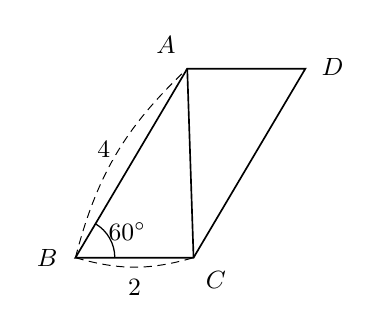
\begin{tikzpicture}[line width=0.6pt, x=1cm, y=1cm]
  \coordinate (A) at (1.42,2.40);
  \coordinate (B) at (0,0);
  \coordinate (C) at (1.50,0);
  \coordinate (D) at (2.92,2.40);
  \draw (A) -- (B) -- (C) -- (D) -- cycle;
  \draw (A) -- (C);
  % 길이 표시의 점선 호
  \draw[densely dashed, line width=0.35pt] (B) to[bend left=16] (A);
  \draw[densely dashed, line width=0.35pt] (B) to[bend right=16] (C);
  % 각 표시
  \draw[line width=0.45pt] (0:0.50) arc (0:59.4:0.50);
  \node[font=\small, fill=white, inner sep=1pt] at (0.36,1.38) {$4$};
  \node[font=\small] at (0.75,-0.38) {$2$};
  \node[font=\small] at (0.66,0.33) {$60^\circ$};
  \node[font=\small, anchor=south east] at (1.40,2.46) {$\pt{A}$};
  \node[font=\small, anchor=east] at (-0.10,0.00) {$\pt{B}$};
  \node[font=\small, anchor=north west] at (1.53,-0.05) {$\pt{C}$};
  \node[font=\small, anchor=west] at (3.00,2.42) {$\pt{D}$};
\end{tikzpicture}
